We look at an interesting approach which needs to be explored further. For long multiplication pattern detection problem, we wish to extract the two operands from the set of partial products. We presented Algorithm \ref{alg:long}, which, given the set of partial products tries to find the corresponding operands, if the partial products indeed represent a long multiplication. 

Consider the following variant of the above stated problem: Given the set of partial products, we wish to extract the multiset of variables in operand1 and operand2 without bothering about the internal ordering of the variables within the operands. The following example looks at it from a graph theoretic point of view.

Given the set of partial products:

\begin{center}

\begin{tabu}{c c c c c}


0 & 0 & $e_1 e_3$ & $e_1 e_3$ & $e_2 e_3$ \\

0 & $e_1 e_1$ & $e_1 e_1$  & $e_1 e_2$ & 0\\

\end{tabu}
\end{center}

We construct an undirected graph G = (V,E) from partial products such that:

\begin{itemize}
\item V = all the unique variables appearing in the partial products
\item V is a set i.e no variable is repeated
\item E = \{$e_i e_j$ $\mid$ $e_i e_j$ or $e_j e_i$ is a partial product\}, one edge per partial product
\item E is a multiset i.e multiple edges and multiple self loops are allowed
\end{itemize}

\begin{figure}

\begin{center}

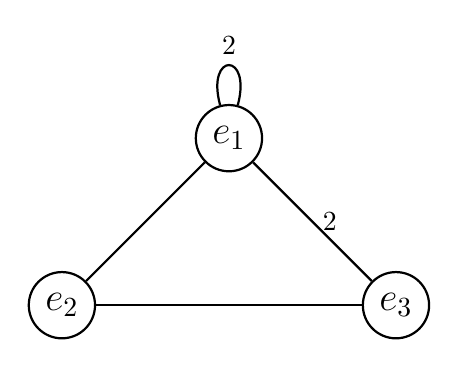
\begin{tikzpicture}[auto, node distance=3cm, every loop/.style={},
                    thick,main node/.style={circle,draw,font=\sffamily\Large\bfseries}]

  \node[main node] (1) {$e_1$};
  \node[main node] (2) [below left of=1] {$e_2$};
  \node[main node] (3) [below right of=1] {$e_3$};

  \path[every node/.style={font=\sffamily\small}];
  \path (1) edge [loop above] node {2} (1);
  \path (3) edge node [right] {} node[right] {2} (1);
  \path (1) edge (2);
  \path (2) edge (3);

\end{tikzpicture}

\caption{Graph G}

\end{center}
\end{figure}

Note - edge weights represent number of edges, default is 1.

\newpage

Question: Is G a complete bipartite graph H = (U,V,E) with the following properties:

\begin{itemize}
\item U can be a multiset
\item V can be a multiset
\item U $\cap$ V need not be empty
\end{itemize}

For the above example, the complete bipartite representation of G that we are looking for is: 
\begin{figure}[h]

\begin{center}

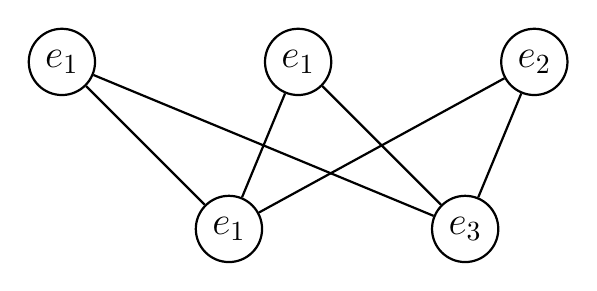
\begin{tikzpicture}[auto, node distance=3cm, every loop/.style={},
                    thick,main node/.style={circle,draw,font=\sffamily\Large\bfseries}]

  \node[main node] (1) {{$e_1$}};
  \node[main node] (2) [right of=1] {{$e_1$}};
  \node[main node] (3) [right of=2] {{$e_2$}};
  \node[main node] (4) [below right of=1] {{$e_1$}};
  \node[main node] (5) [below right of=2] {{$e_3$}};
  
  \path[every node/.style={font=\sffamily\small}];
  \path (1) edge  (4);
  \path (1) edge  (5);
  \path (2) edge  (4);
  \path (2) edge  (5);
  \path (3) edge  (4);
  \path (3) edge  (5);

\end{tikzpicture}
\caption{Graph H}

\end{center}
\end{figure}

The problem of finding whether a graph G is a complete bipartite graph under the given conditions is equivalent to finding the factors(if they exist) of a multivariate polynomial of degree 2 with no constant terms. The polynomial corresponds to the graph G whereas the factors correspond to each partition of graph H. For the above example, the multivariate polynomial is:
$(2 e_1^2 + e_1e_2 + e_2e_3 + 2 e_1e_3)$. The factors for this polynomial are $(2 e_1 + e_2)$ and $(e_1 + e_3)$.

Solving the above stated problem would give us the variables present in each operand of the long multiplication. However, we still would not know the ordering of the variables(if it exists) i.e concatenation order of the variables within the operands. We are still exploring this approach as part of our future work.
